\section{پیاده‌سازی کنترل‌کننده برای کنترل کانال رول-پیچ}\label{roll_pitch_lqidg_section}
در بخش
\ref{roll_pitch_lqidg_section_simulation}
شبیه‌سازی کانال رول-پیچ استند چهارپره در حضور کنترل‌کننده \lr{LQIDG} انجام شد. در این بخش به پیاده‌سازی کنترل‌کننده \lr{LQIDG} بر رویه کانال رول-پیچ استند سه درجه آزادی پرداخته می‌شود.
در پیاده‌سازی از ضرایب وزنی بهینه به دست آمده در قسمت شبیه‌سازی استفاده شده‌است.

\begin{figure}[H]
	\centering
	\subfigure[تغییرات زاویه رول]{
		\centering
		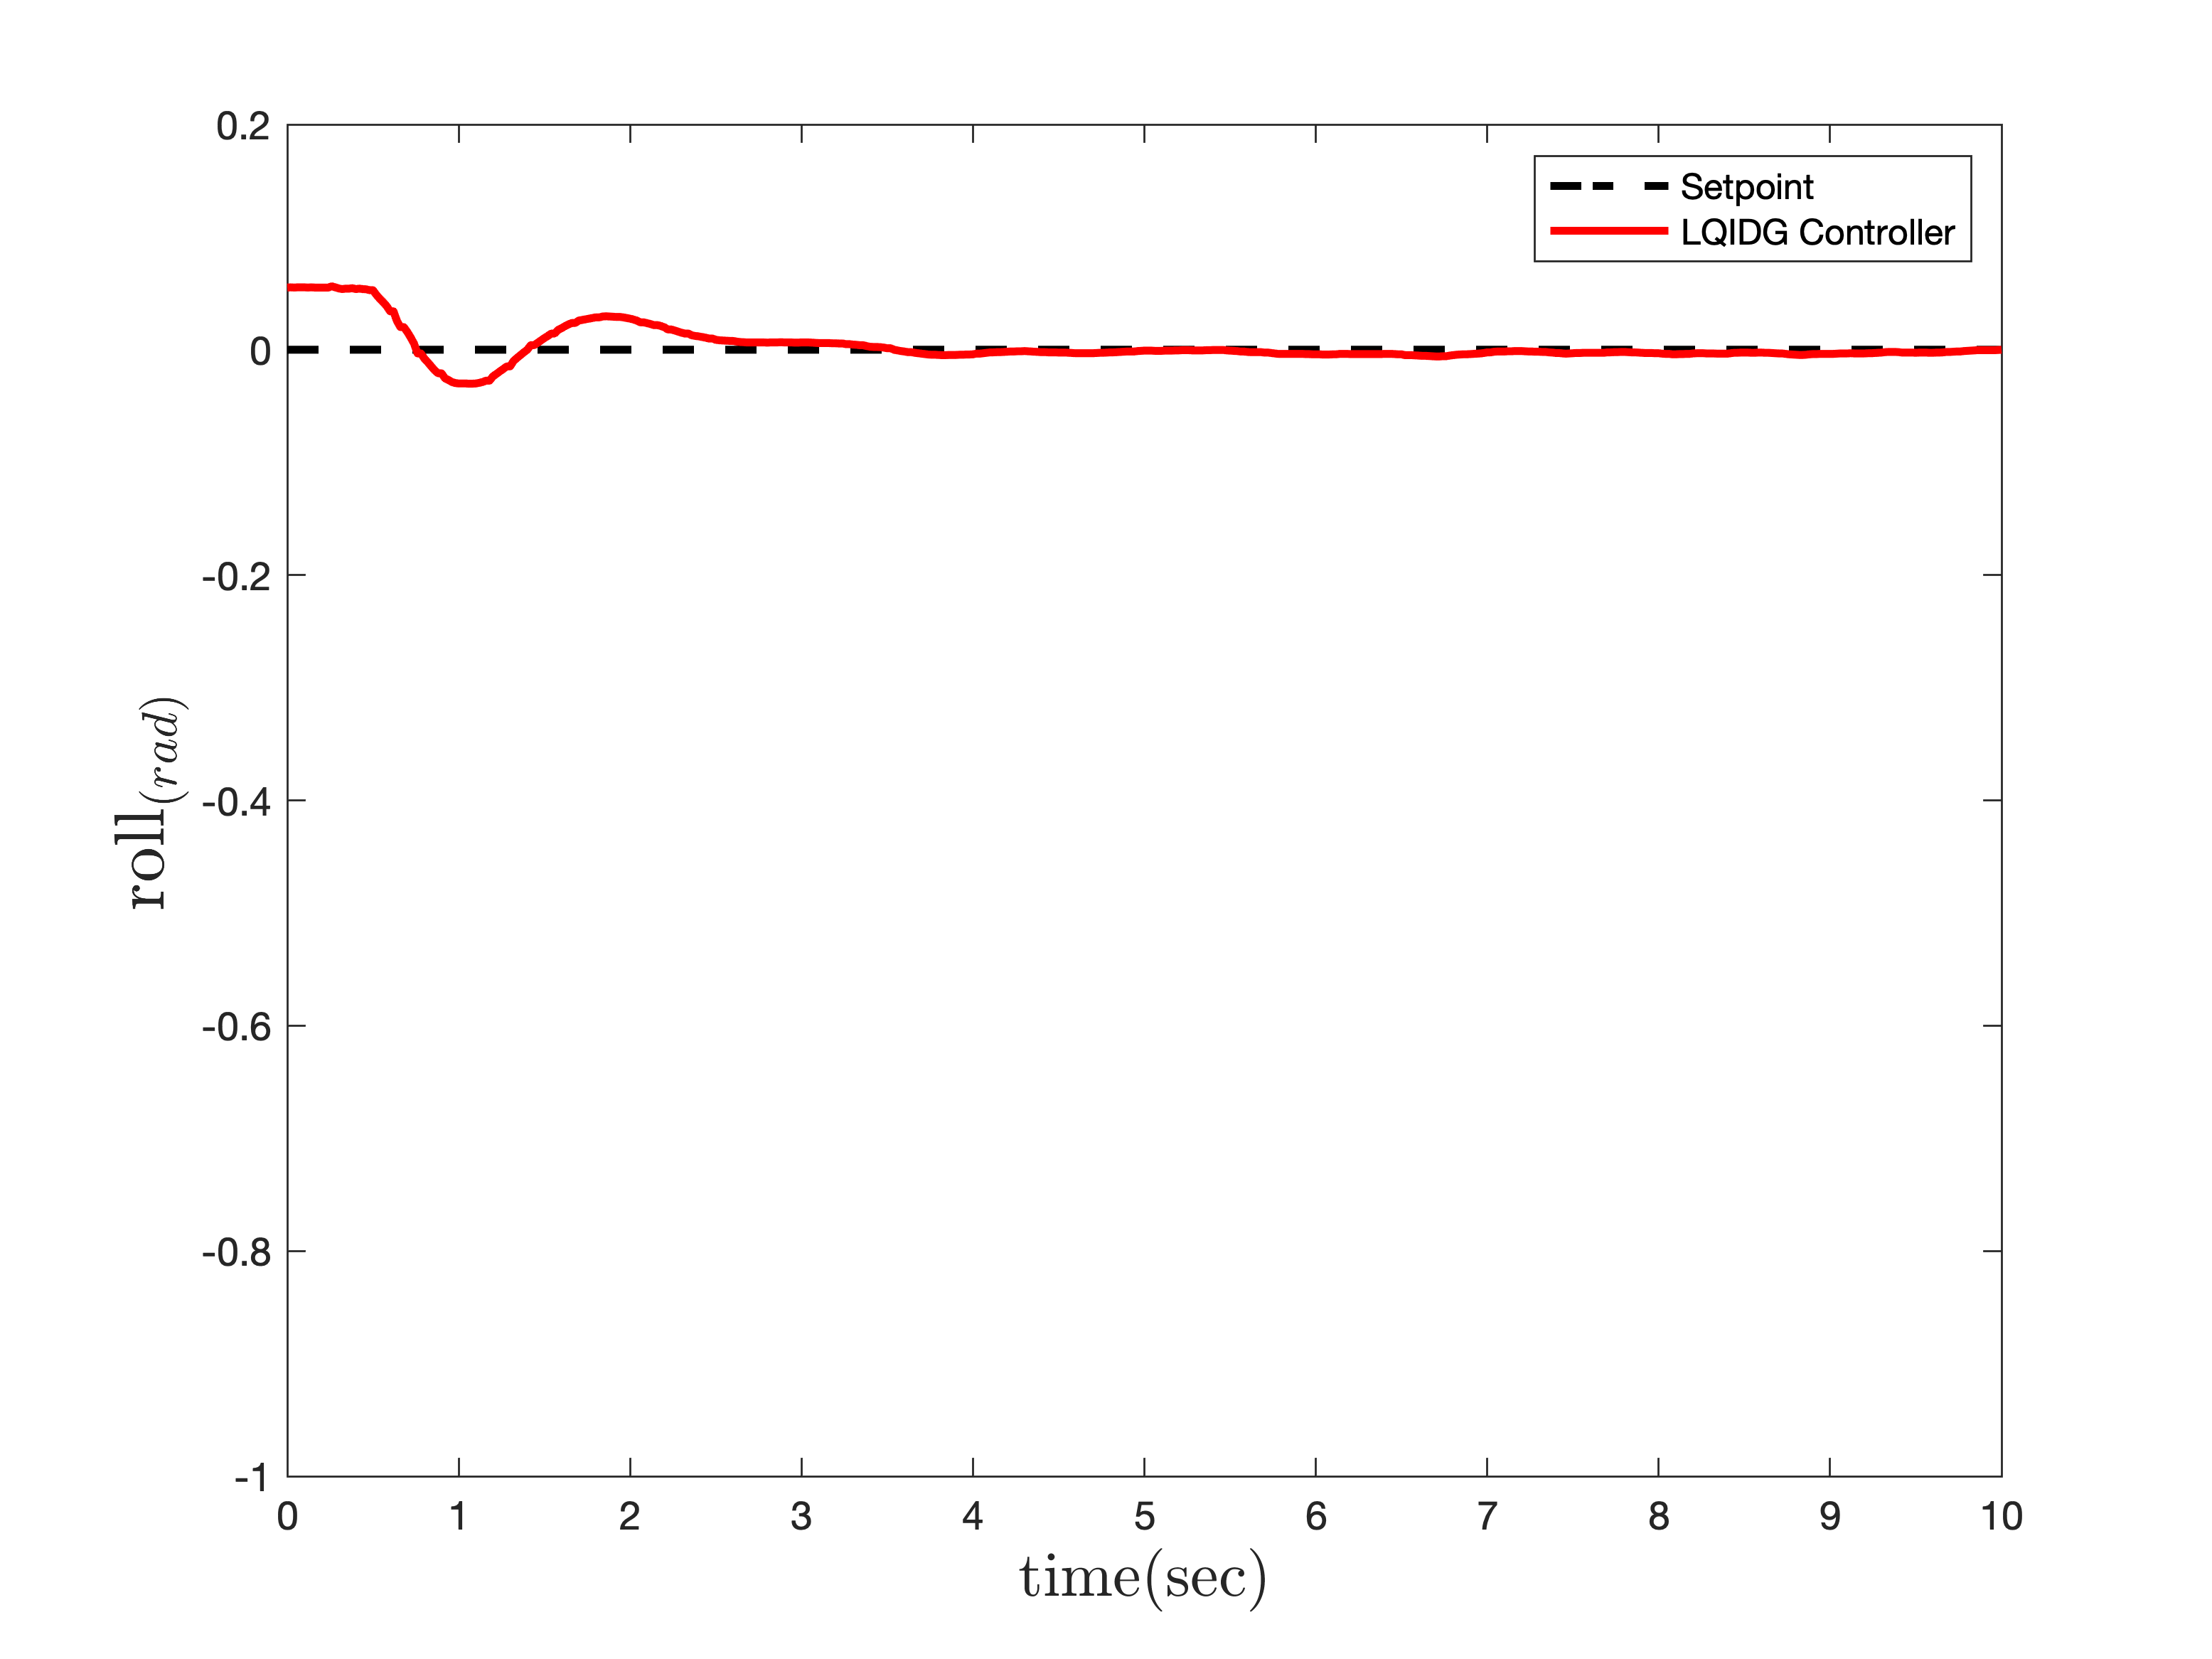
\includegraphics[width=.48\linewidth]{../Figures/Calibration/LQIDG/Roll_Pitch/lqidg_roll.png}
	}
	\subfigure[تغییرات زاویه پیچ]{
		\centering
		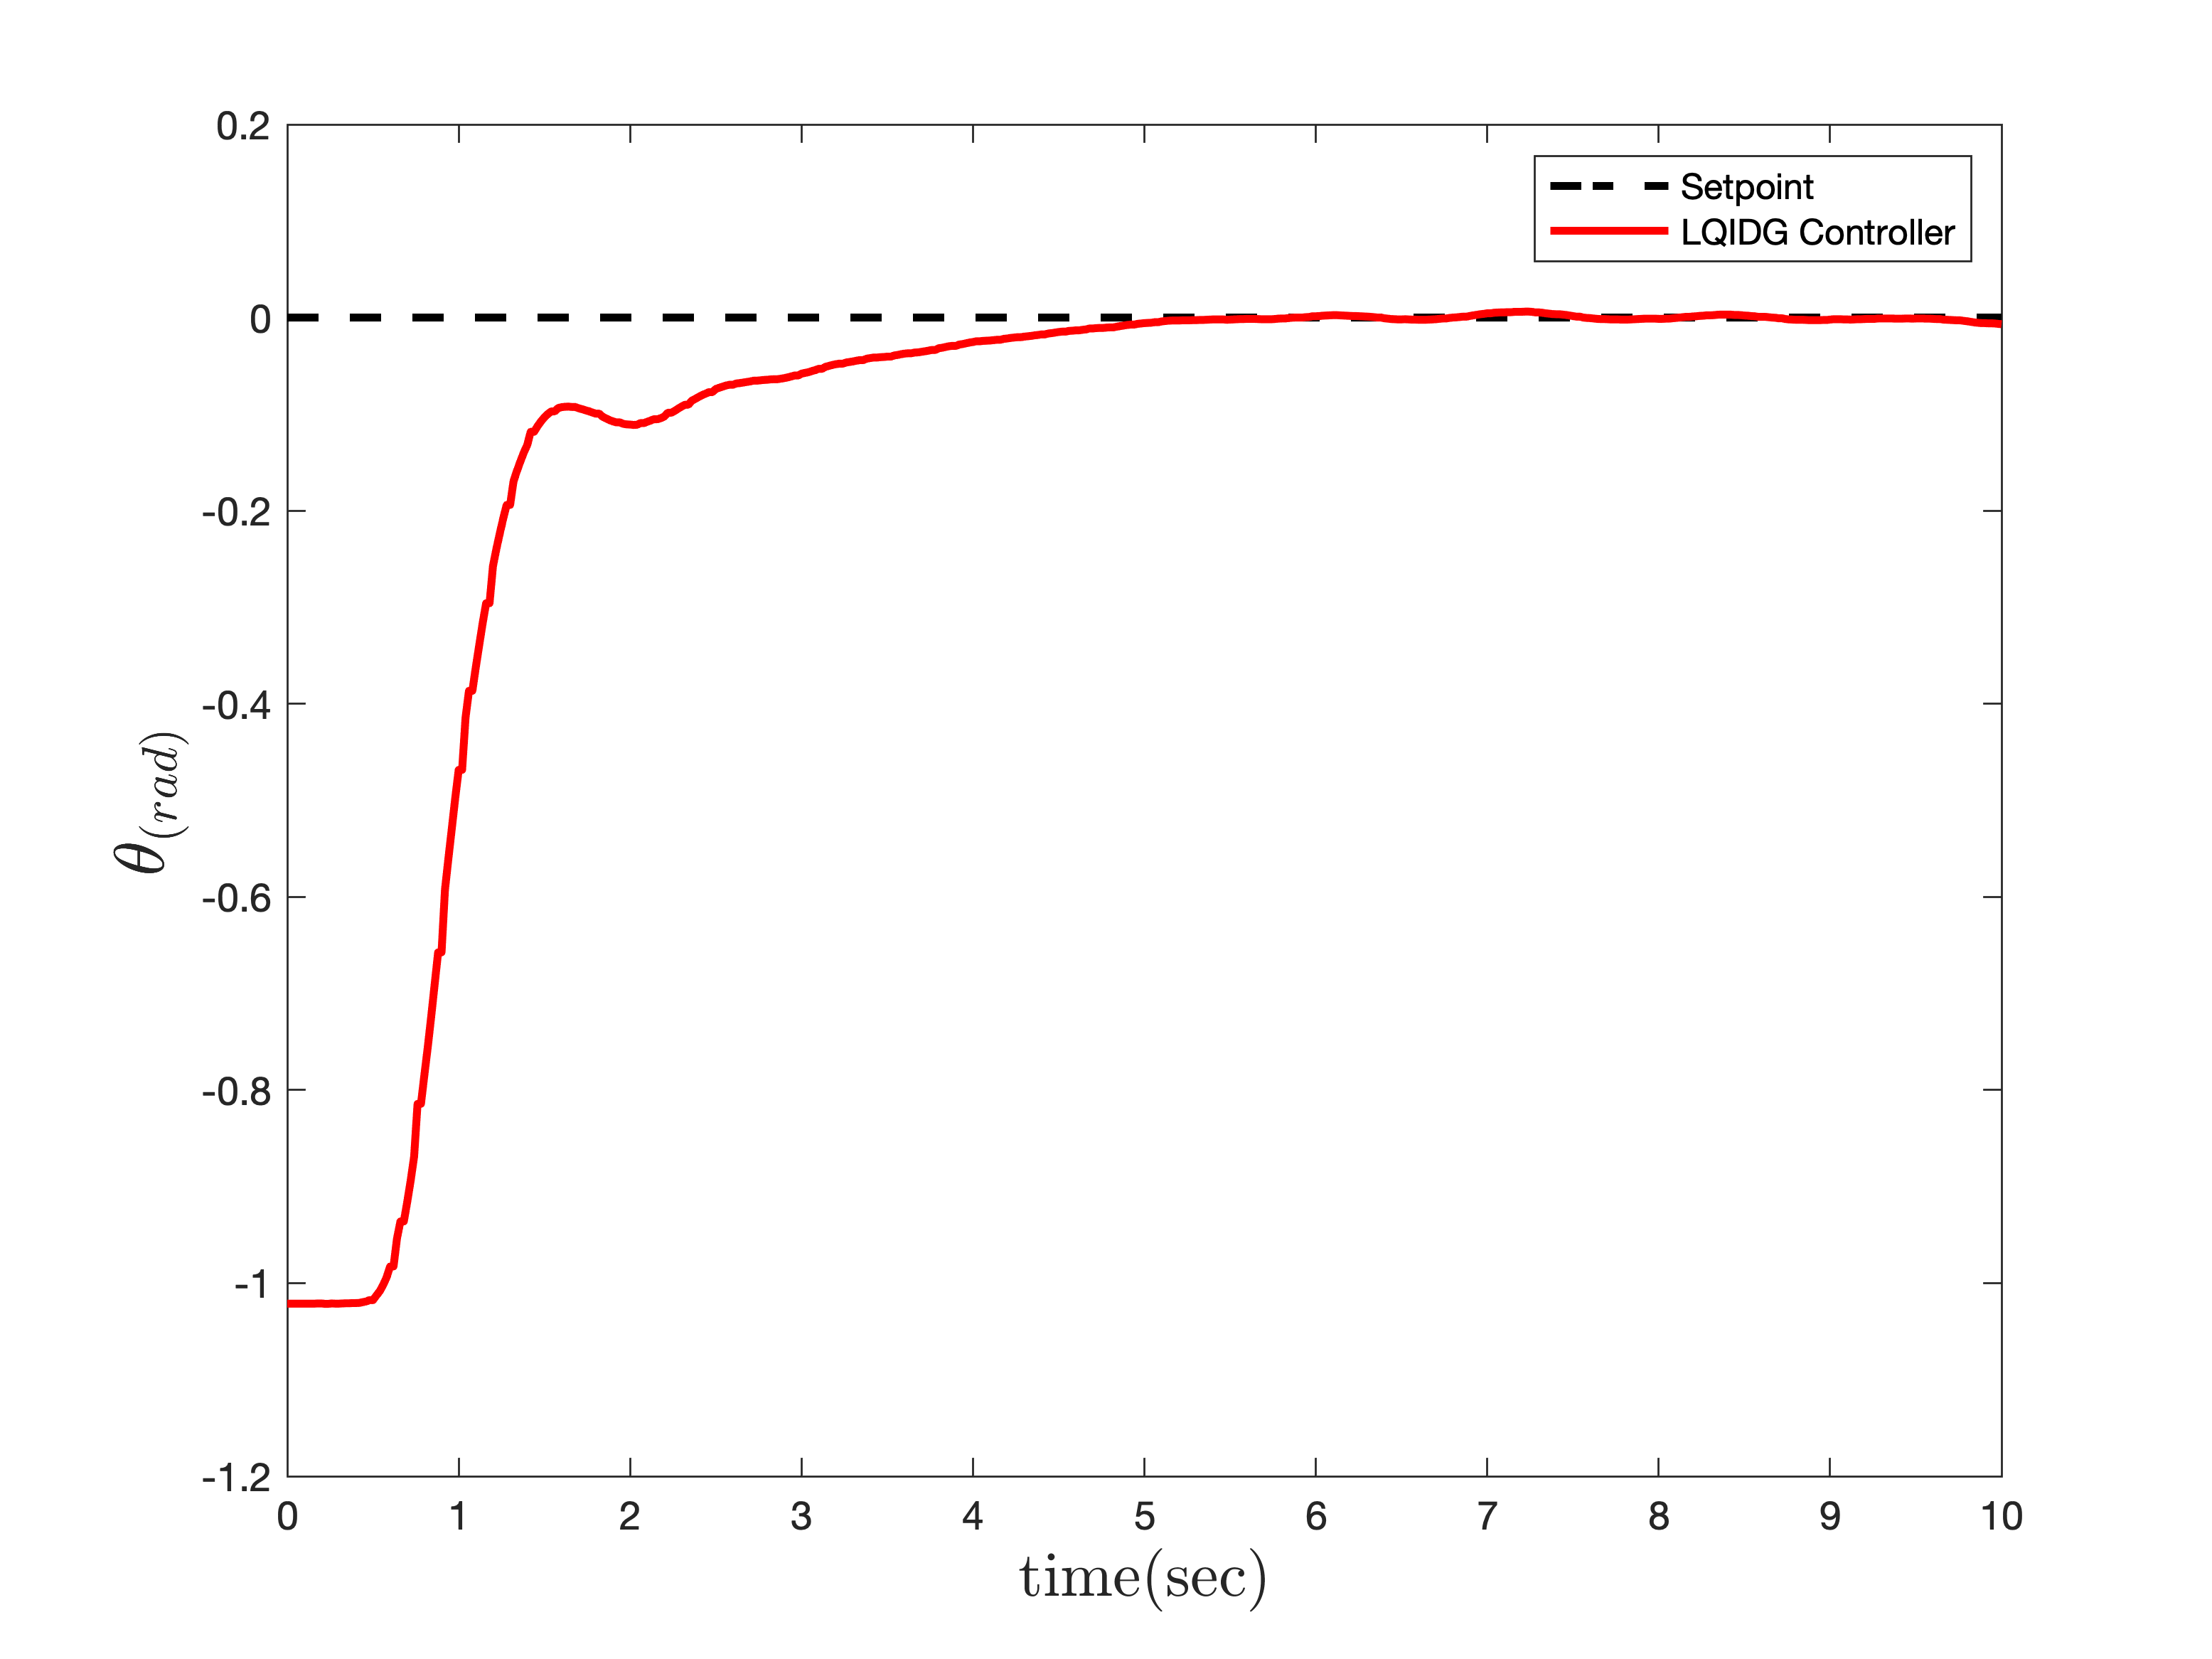
\includegraphics[width=.48\linewidth]{../Figures/Calibration/LQIDG/Roll_Pitch/lqidg_pitch.png}
	}
	\caption{‫‪عملکرد کنترل‌کننده \lr{LQIDG} در کنترل زاویه رول و پیچ (تعقیب ورودی صفر)}
\end{figure}

\begin{figure}[H]
	\centering
	\subfigure[موتور شماره یک]{
		\centering
		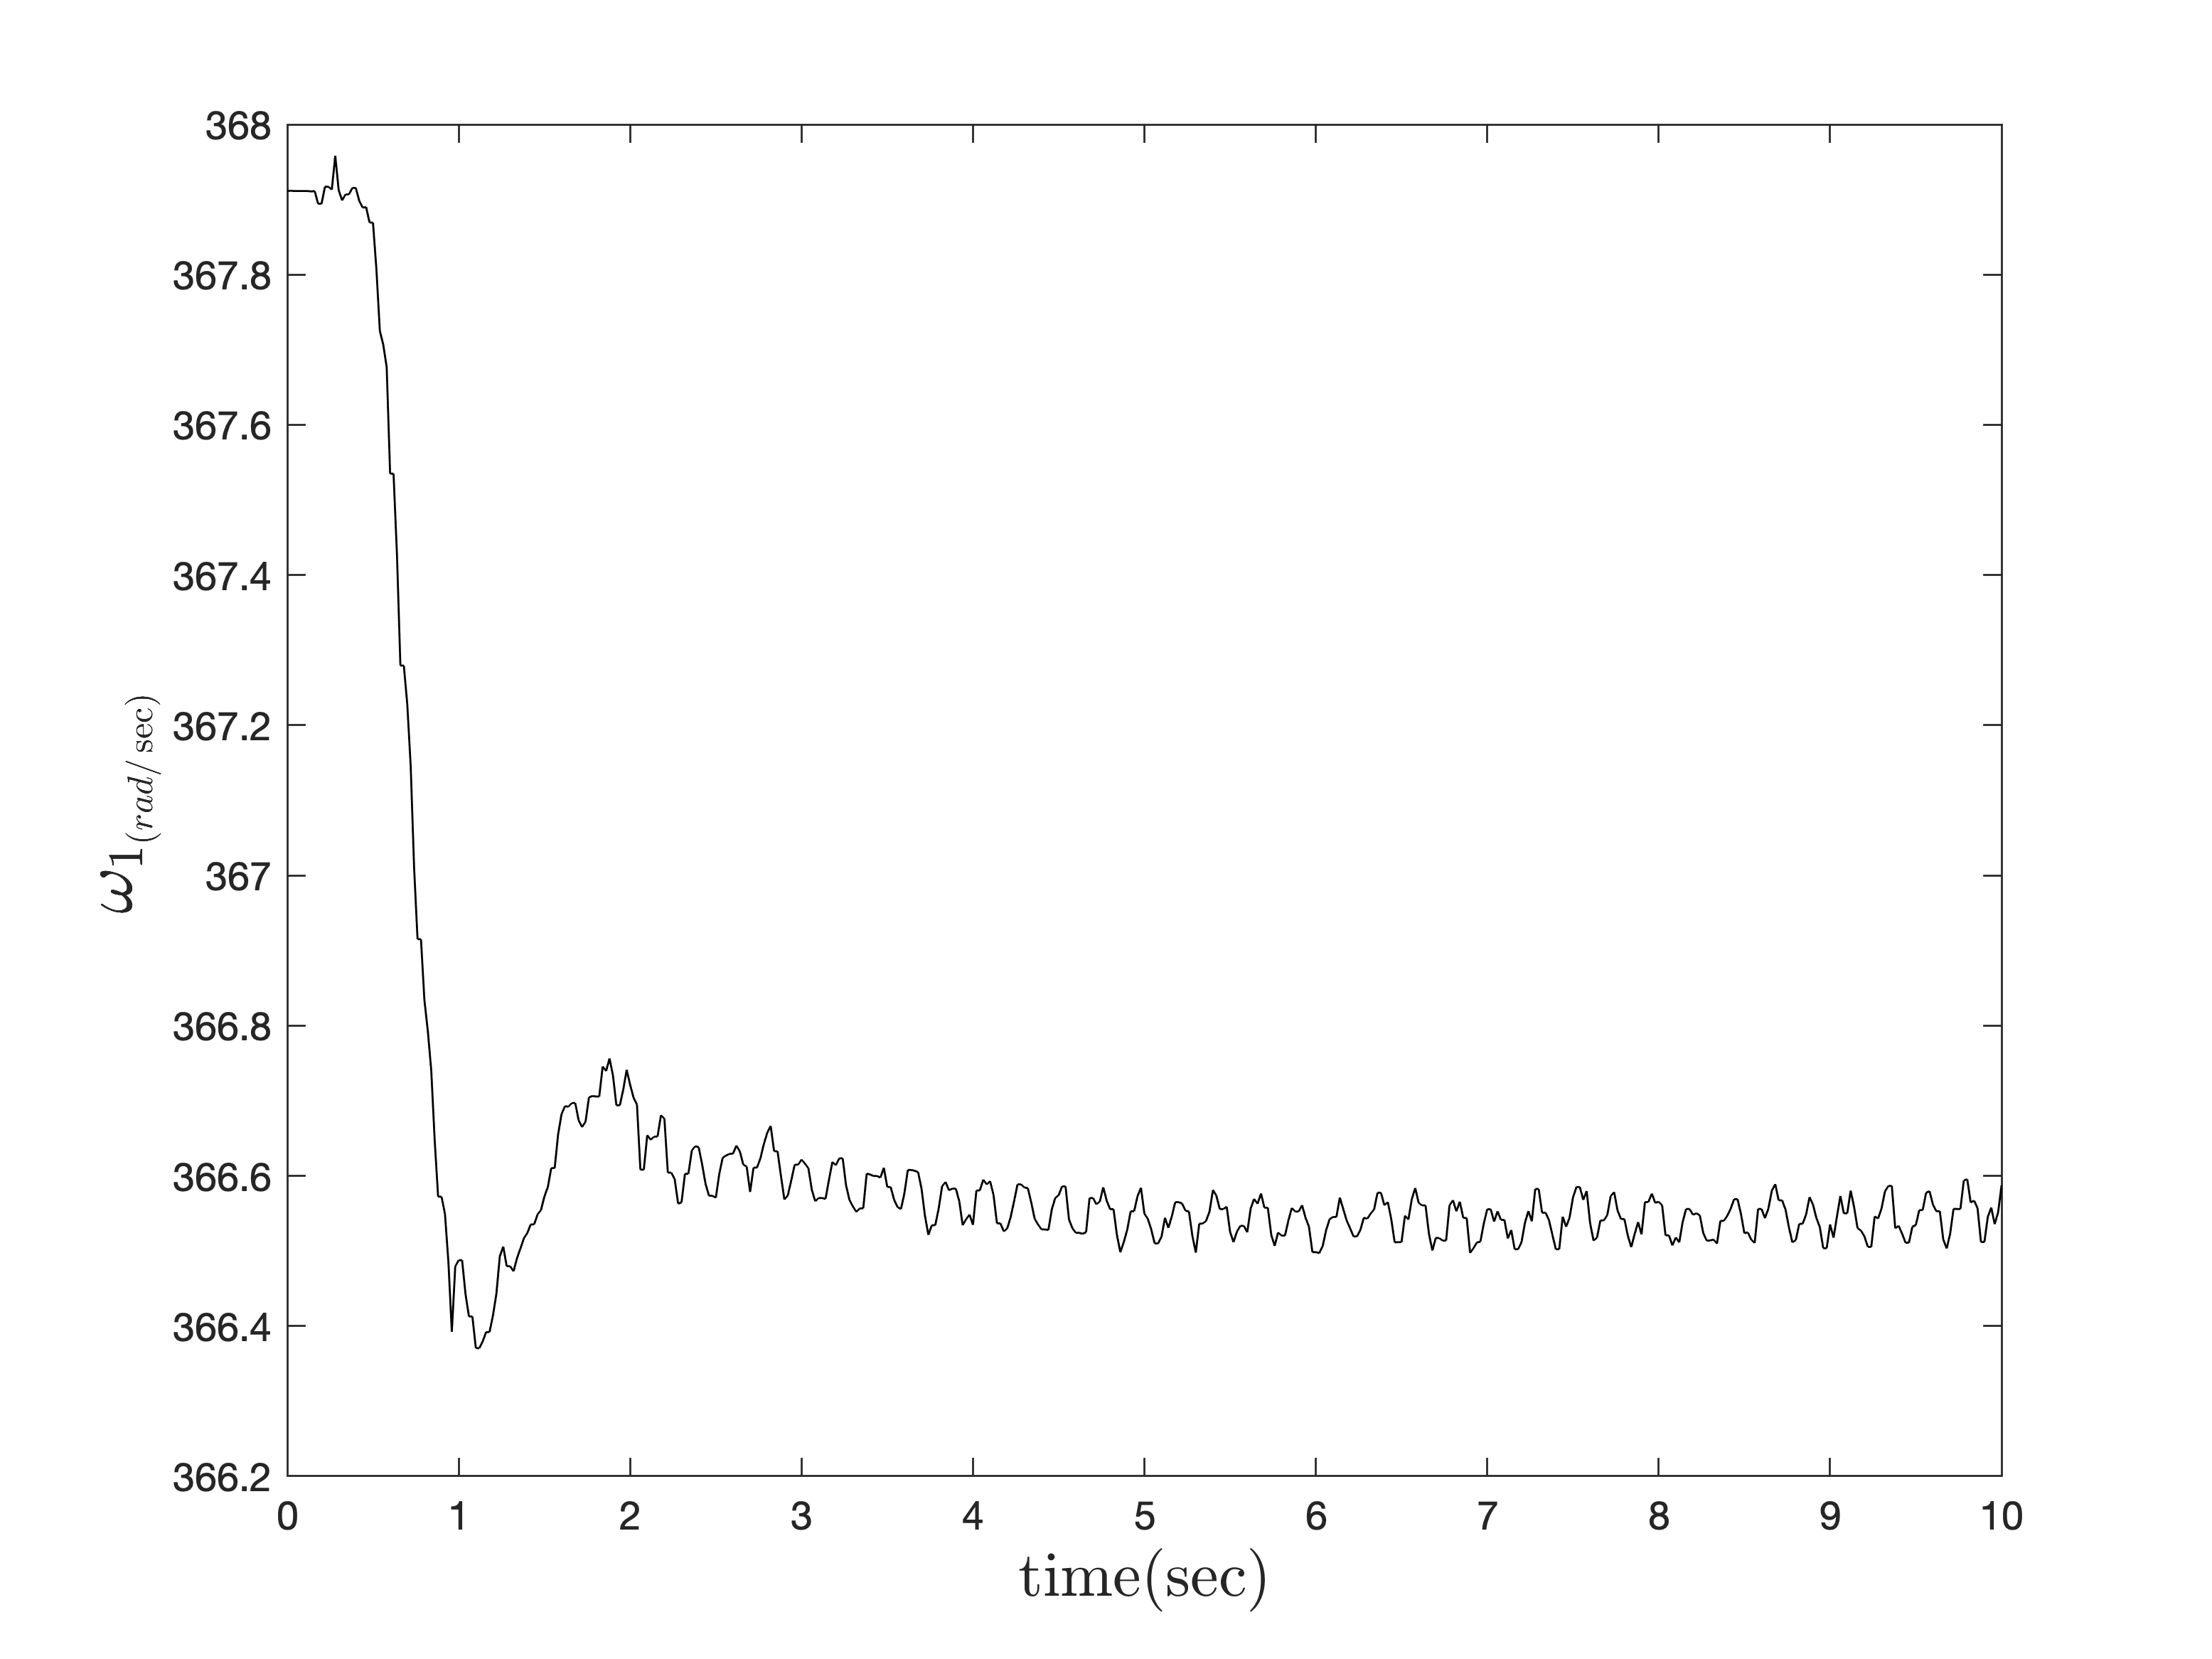
\includegraphics[width=.45\linewidth]{../Figures/Calibration/LQIDG/Roll_Pitch/lqidg_Omega_1.png}
	}
	\subfigure[موتور شماره دو]{
		\centering
		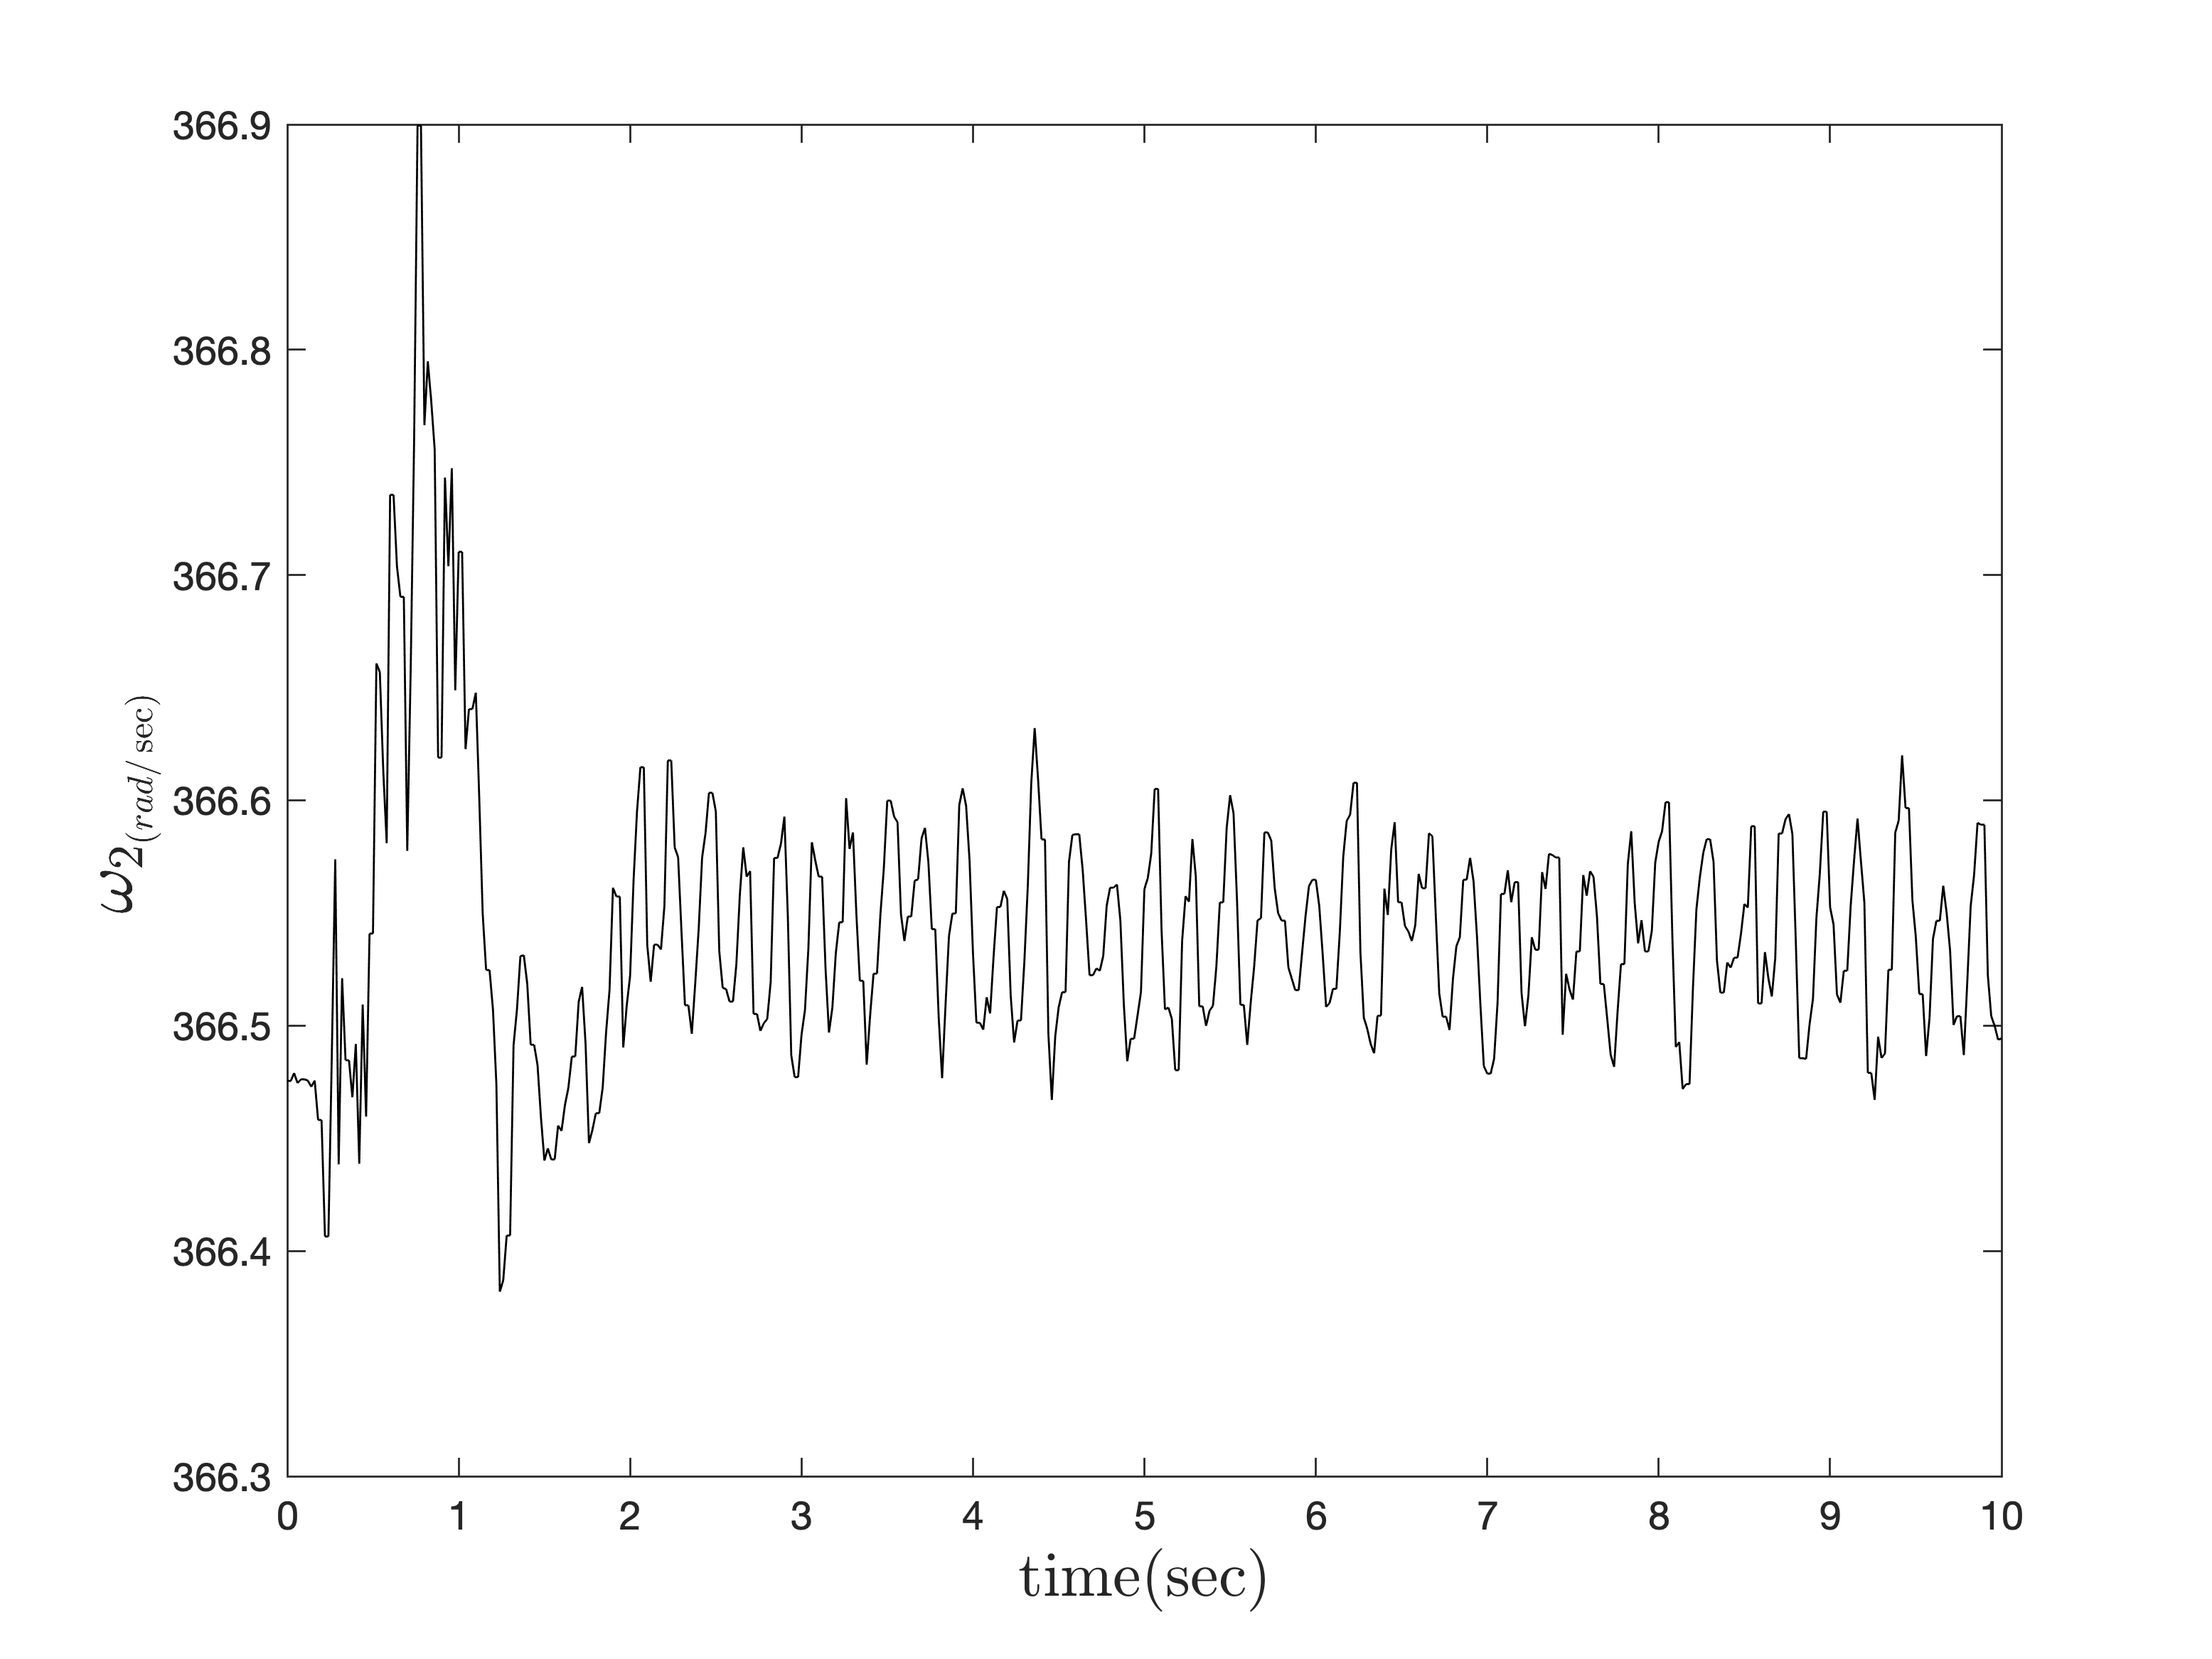
\includegraphics[width=.45\linewidth]{../Figures/Calibration/LQIDG/Roll_Pitch/lqidg_Omega_2.png}
	}
	\subfigure[موتور شماره سه]{
		\centering
		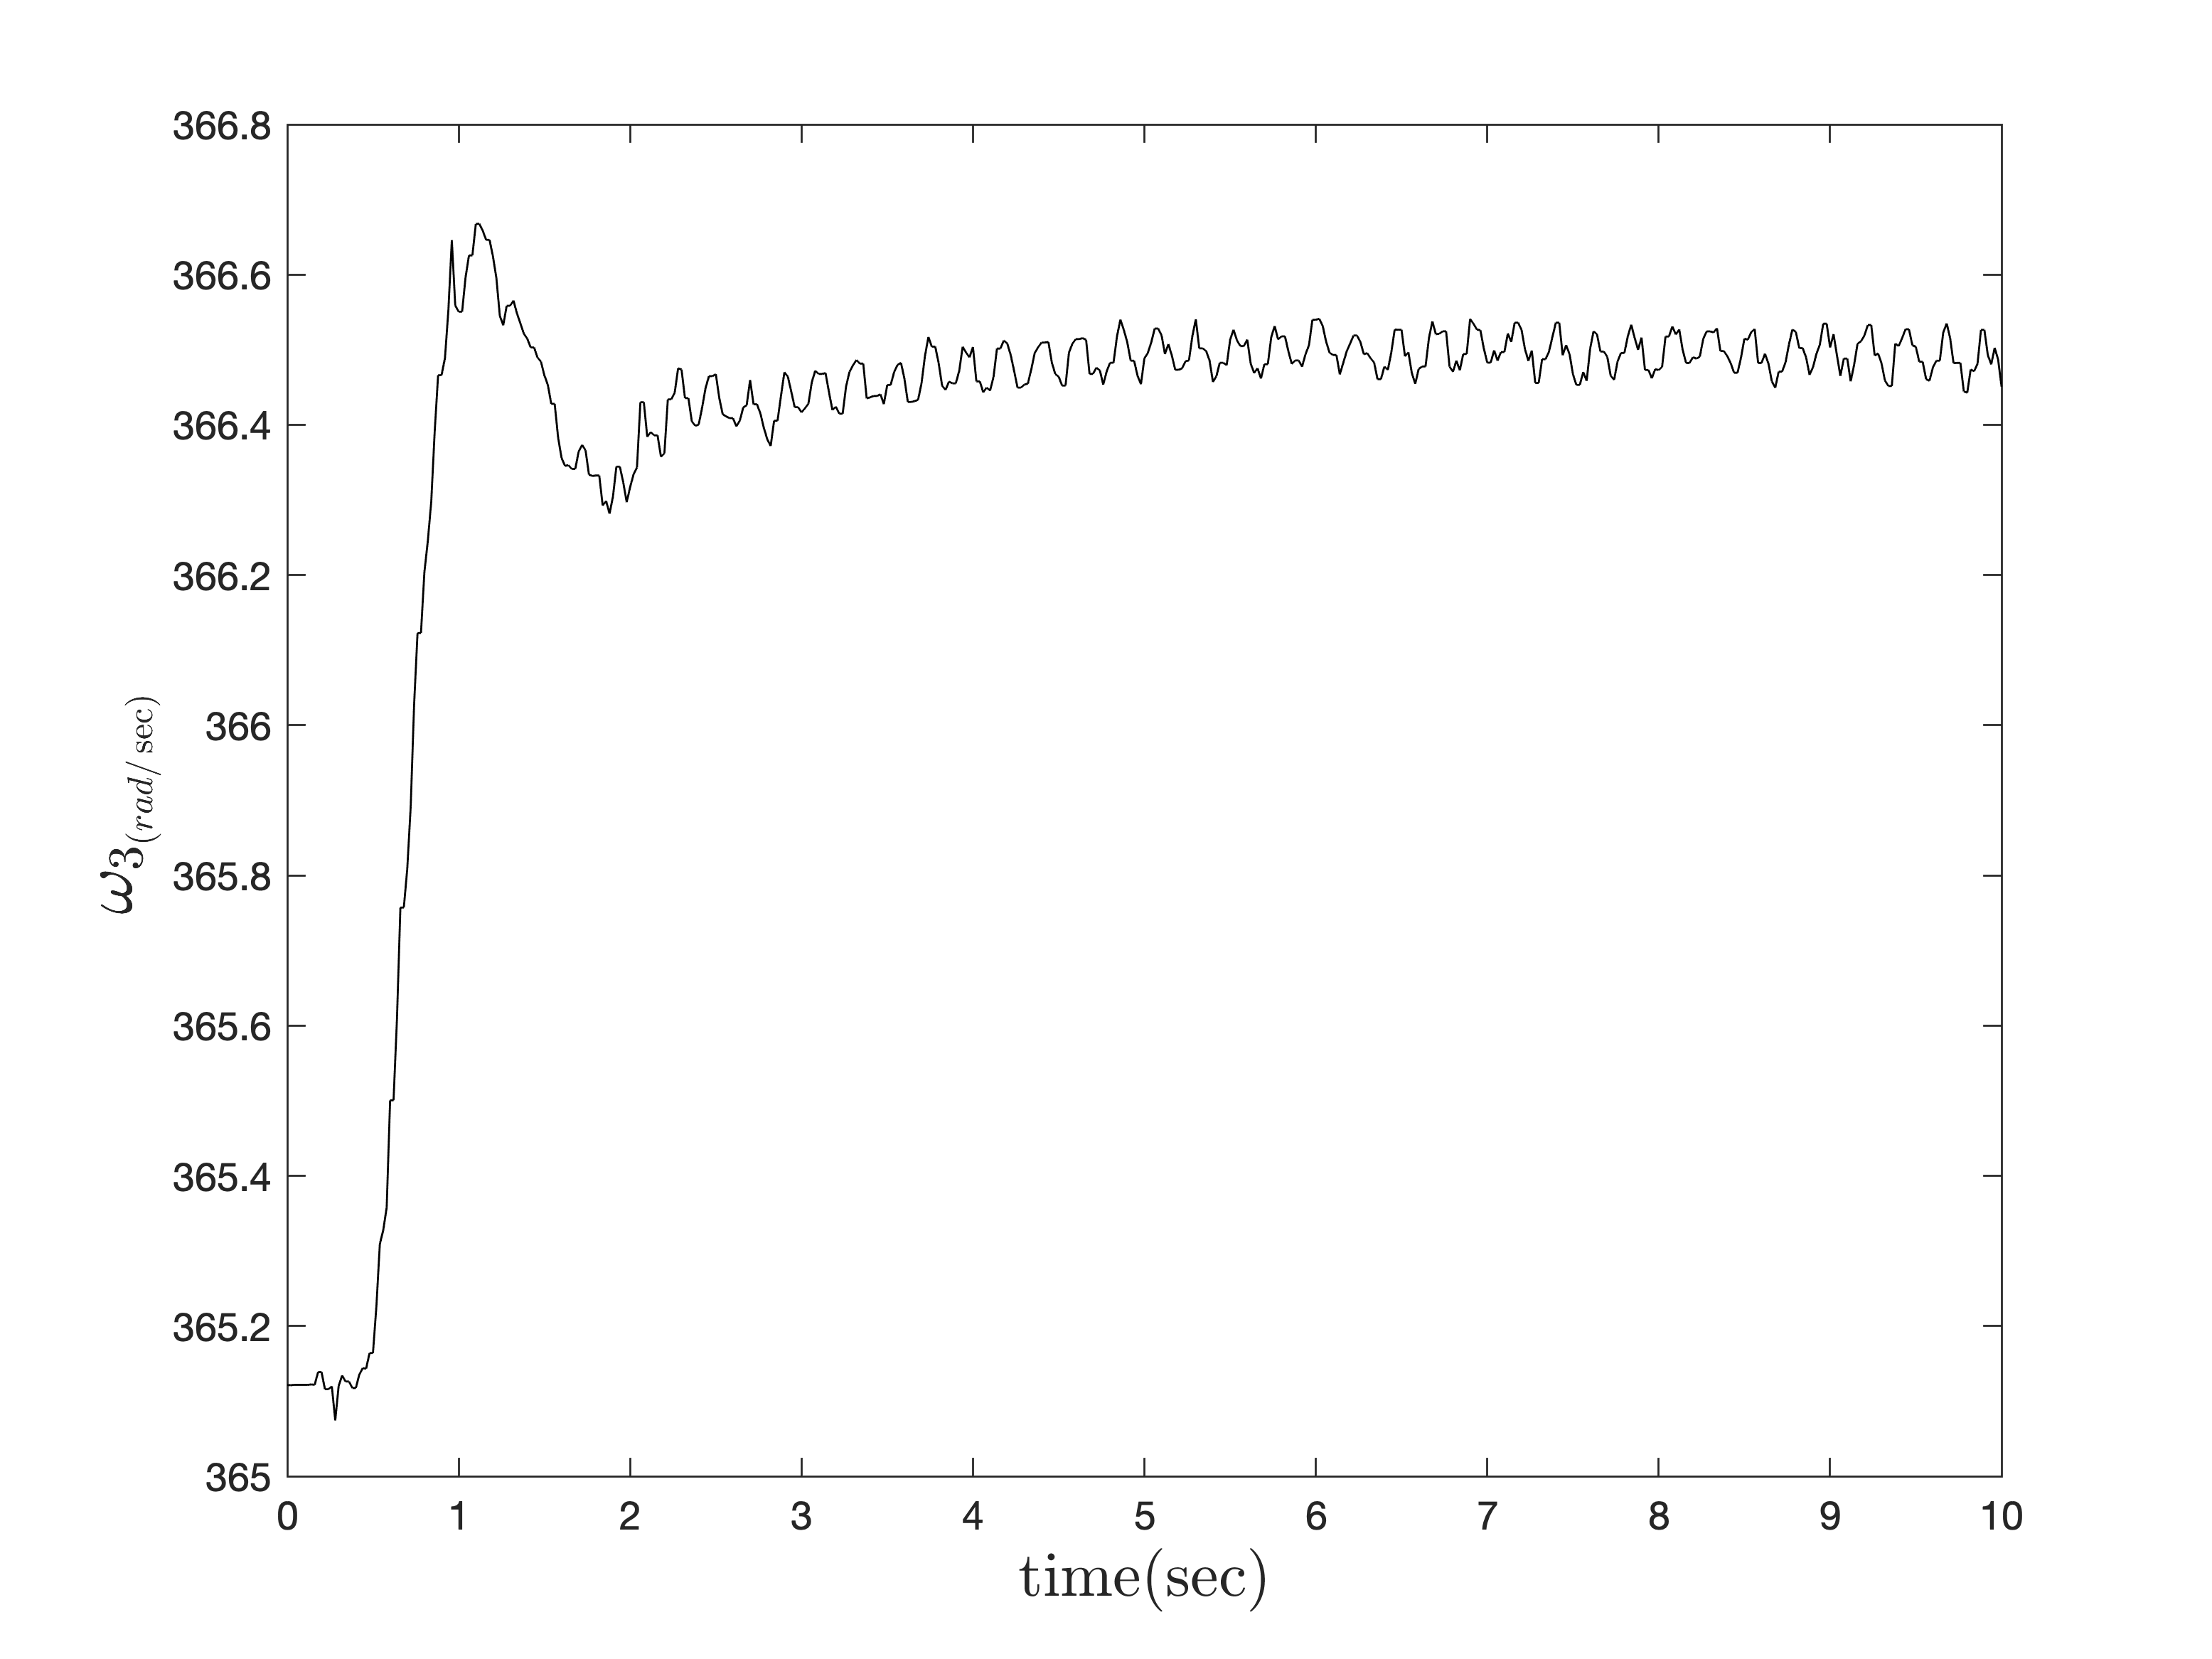
\includegraphics[width=.45\linewidth]{../Figures/Calibration/LQIDG/Roll_Pitch/lqidg_Omega_3.png}
	}
	\subfigure[موتور شماره چهار]{
		\centering
		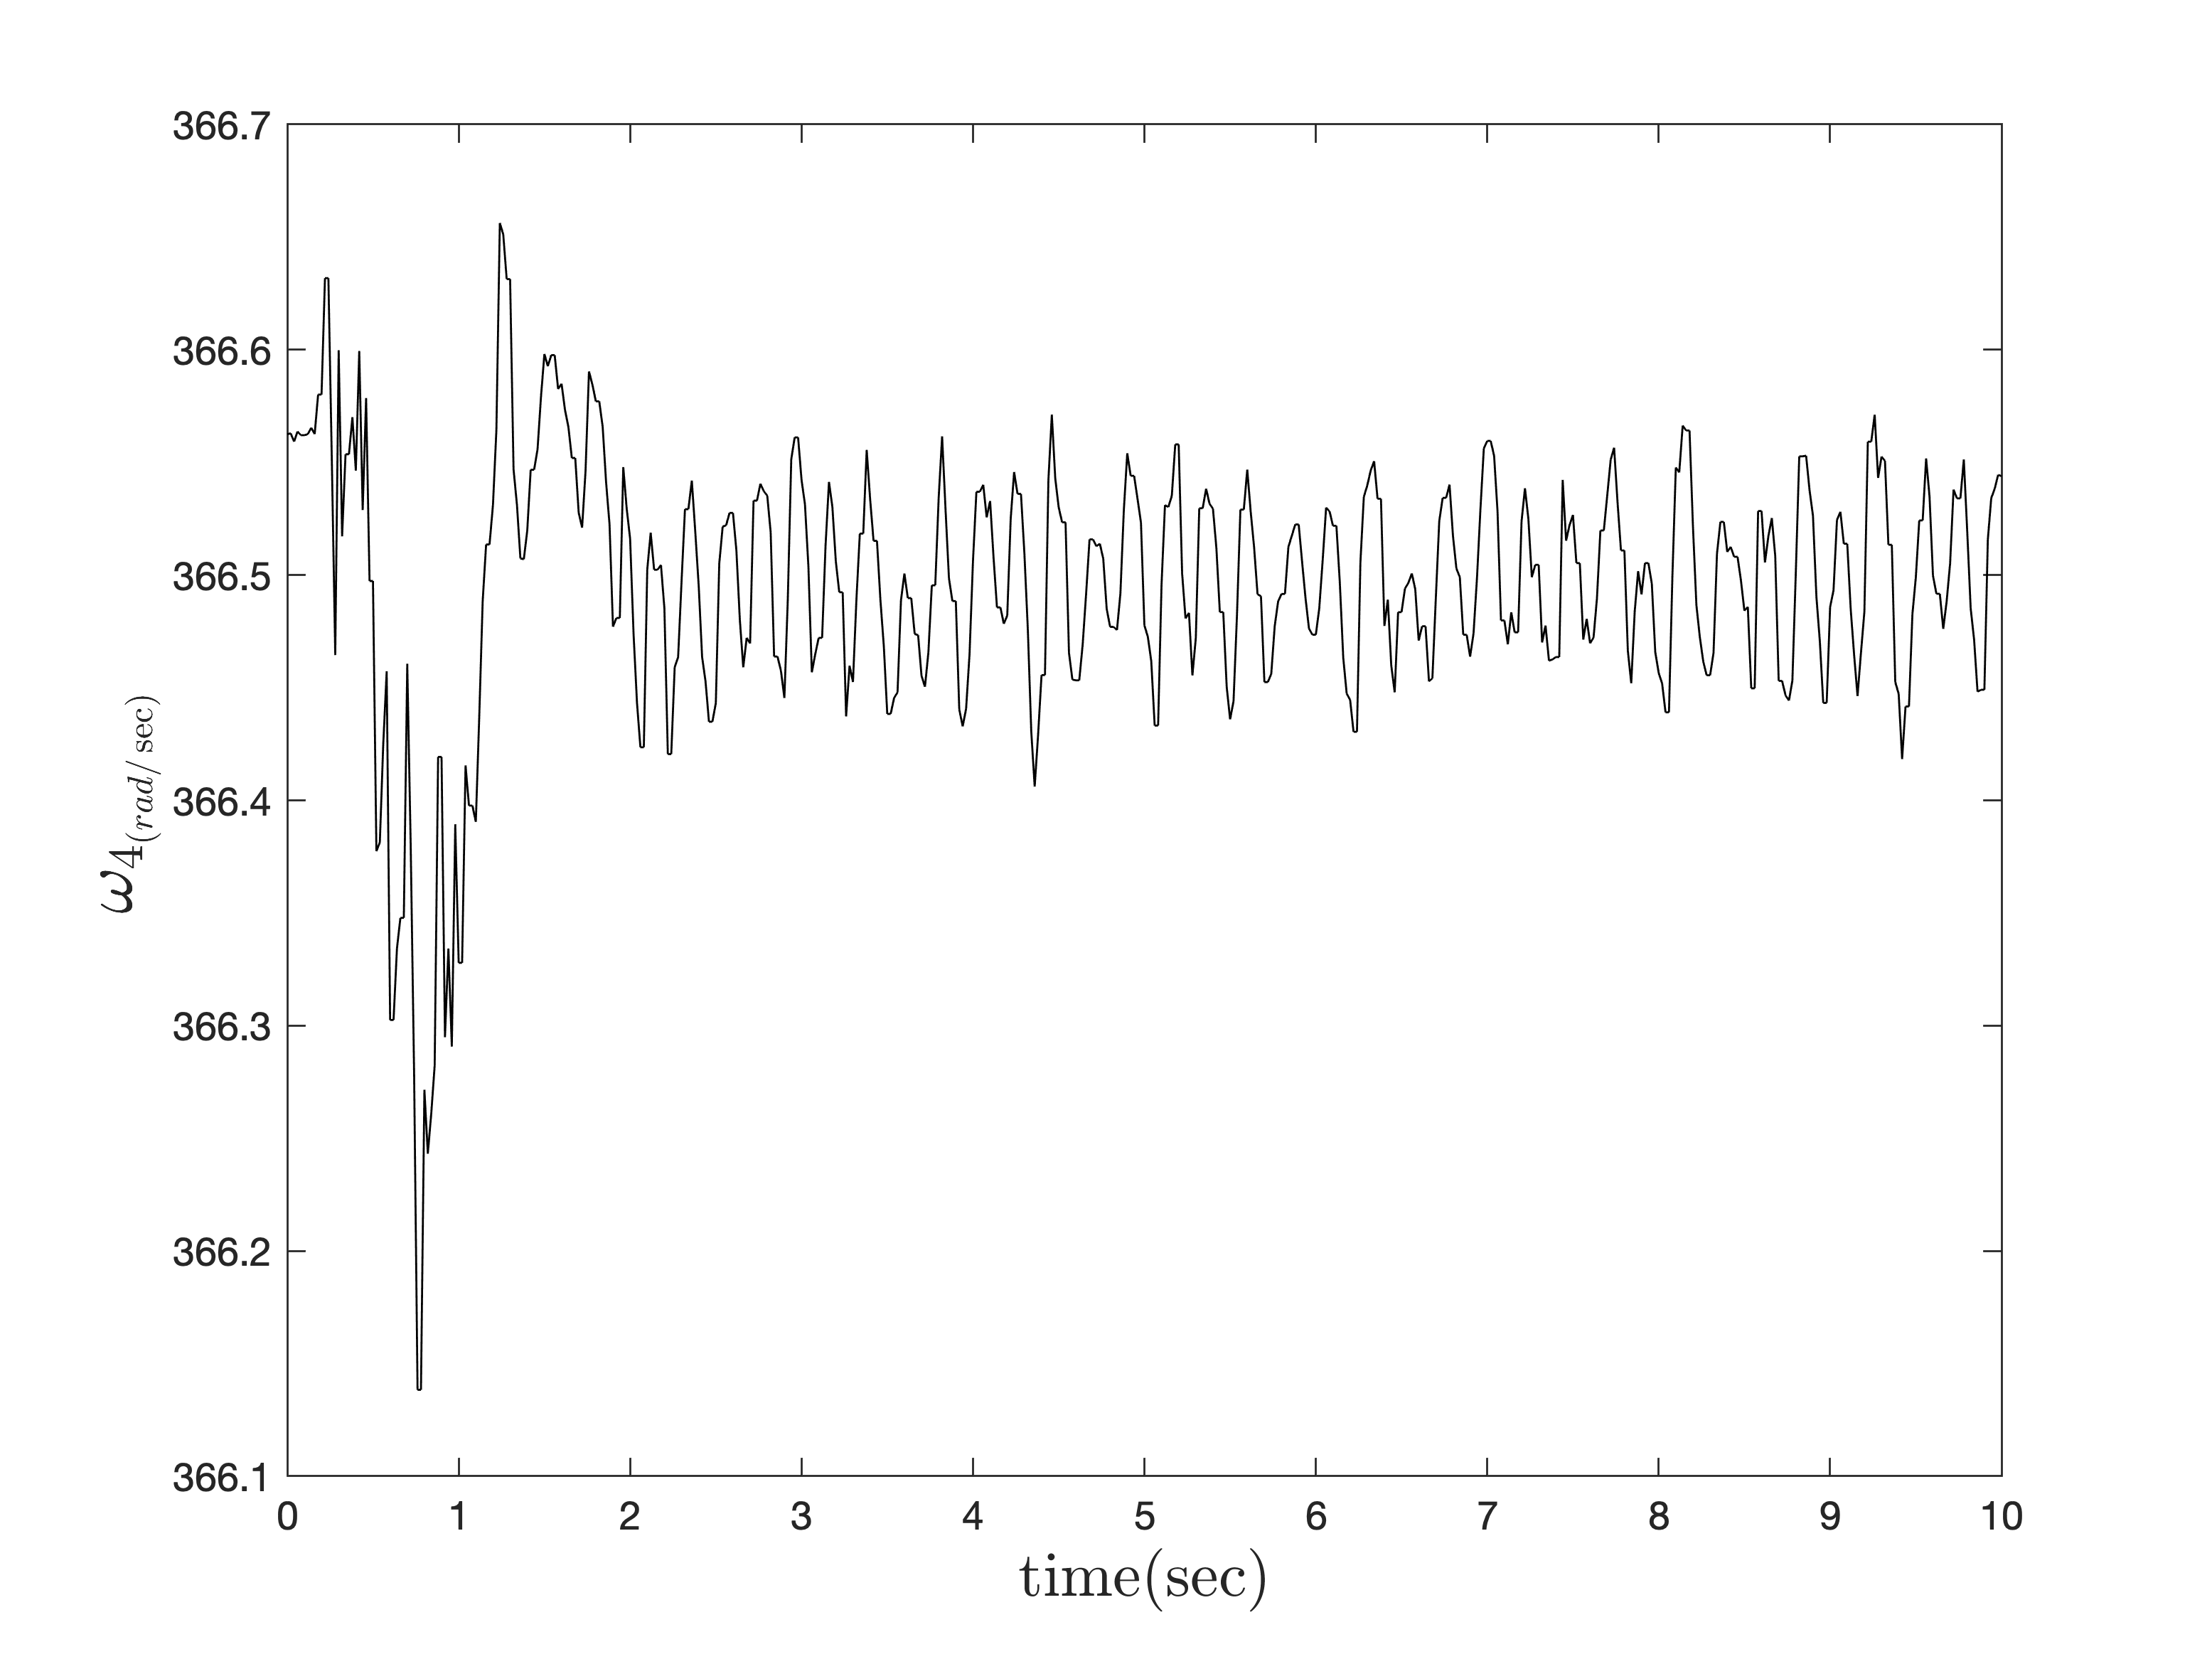
\includegraphics[width=.45\linewidth]{../Figures/Calibration/LQIDG/Roll_Pitch/lqidg_Omega_4.png}
	}
	\caption{‫‪فرمان کنترلی موتورها در کنترل زاویه رول و پیچ (تعقیب ورودی صفر)}
\end{figure}






%بر اساس خروجی شبیه‌سازی (شکل
%\ref{lqidg_roll_fig})
%،کانال رول در حضور کنترل‌کننده \lr{LQIDG} در حدود پنج ثانیه و کانال پیچ در حدود هشت ثانیه به تعادل می‌رسد و خطای ماندگار آن در حدود صفر است.